\documentclass[12pt, a4paper]{article}
\usepackage{../notesheets}
%%%%%%%%%%%%%%%%%%%%%%%%%%%%%%%%%%%%%%%%%%%%%%%%%% 
\author{Math 1220}
\title{Notesheet. Section 8.3 Part 2: Maxima and Minima of Function of
  Several Variables}
\date{}

\begin{document}
\maketitle
\nameline
%%%%%%%%%%%%%%%%%%%%%%%%%%%%%%%%%%%%%%%%%%%%%%%%%%
\vspace{-0.3in}
\begin{ex}
  Consider the function \(f(x,y) = (1-x^2) \sin(y)\). Compute the
  following
  \begin{enumerate}
  \item \(f_x(0,0), f_y(0,0)\) and \(f_x(1,0),f_y(1,0)\).
    \vspace{0.75in}
  \item \(f_{xx}(0,0), f_{xy}(0,0), \) and \(f_{yy}(0,0)\)
    \vspace{0.75in}
  \item \(f_{xx}(1,0), f_{xy}(1,0),\) and \(f_{yy}(1,0)\)
  \end{enumerate}
\end{ex}
\vspace{-1.5in}
\begin{thrm}[The Second Derivative Test]
  Let \(f(x,y)\) be a twice differentiable function with continuous
  second derivatives. Let \[
    D(a,b) = f_{xx}(a,b)f_{yy}(a,b) - [f_{xy}(a,b)]^2
  \]
  If \(f_x = 0\) and \(f_y = 0\),
  \begin{enumerate}[label=(\alph*)]
  \item \(D(a,b) > 0\) and \(f_{xx}(a,b) < 0\), then
    \vspace{0.075in}
  \item \(D(a,b) > 0\) and \(f_{xx}(a,b) > 0\), then
    \vspace{0.075in}
  \item \(D(a,b) < 0\), then
    \vspace{0.075in}
  \item \(D(a,b) = 0\), then
  \end{enumerate}
\end{thrm}
\vspace{-0.5in}
\begin{ex}
  Use the second derivative test to determine \(f(x,y) =
  (1-x^2)\sin(y)\) classify the which type of critical point \((0,0)\) and
  \((1,0)\) are.
\end{ex}
\begin{ex}
  Let \(f(x,y) = x^3-6xy+y^2\). find and classify all the critical
  points of \(f(x,y)\).
\end{ex}
\begin{ex}
  Find the dimensions that minimized the material used to construct an
  open rectangular box having a fixed volume 
  of \(32\) cubic inches.
  \\ 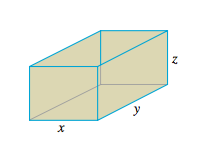
\includegraphics[scale=0.75]{images/open-box}
\end{ex}
\begin{ex}
  Find the point \((x,y)\) such that the sum of the distances squared
  from \((x,y)\) to \((0,0), (2,1), (0,3)\) is minimized. Hint:
  remember the distance formula from the Pythagorean theorem: \(d^2 =
  (x-x_0)^2 + (y-y_0)^2\).
\end{ex}
%%%%%%%%%%%%%%%%%%%%%%%%%%%%%%%%%%%%%%%%%%%%%%%%%% 
\end{document}